\section{Mathematical Notation}
\label{mathematical_notation}

\paragraph{Note about the current state of the documentation}
It would be nice for some laws (like the commutative law of addition in arithmetic) to be included, but this will not be part of the first iteration of the documentation. The Z reference manual does this.
References to related proof rules would be nice to have too, but again, this is not part of the first iteration.

\subsection{Introduction}
\label{mathematical_notation_introduction}

\subsubsection{Data types}
\label{data_types}

In Event-B we have 3 kinds of basic data types:
\begin{itemize}
\item $\intg$ is the set of all integers.
\item \index{boolean!as type}
  $\Bool$ is the set of Booleans. 
  It has two elements $\Bool = \{\True,\False\}$.
\item User defined carrier sets. 
  These are defined in the \eventbsection{Sets} section of a context.
  Carrier sets are never empty.
  There is no other assumption made about carrier sets unless it is stated explicitly as
  an axiom.
\end{itemize}
From all data types $\alpha, \beta$, two other kinds of data types can be constructed:
\begin{itemize}
\item $\pow(\alpha)$ contains the sets of elements of $\alpha$.
\item $\alpha\cprod\beta$ contains the pairs where the first element is of type $\alpha$ and the
  second element of type $\beta$.
\end{itemize}
\paragraph{A note about the notation}
We use the Greek letters $\alpha$, $\beta$, $\gamma$, \ldots to represent arbitrary data types.
For an expression $E$, we write $E\in\alpha$ to state that $E$ is of type $\alpha$.
In the following descriptions of Event-B's mathematical construct we describe the
  types of all constructs and their components.

For example, we will describe the maplet $E\mapsto F$ which is defined as $E\mapsto F\in\alpha\cprod\beta$ with
 $E\in\alpha$ and $F\in\beta$. We do not make any restrictions on the types $\alpha$ and $\beta$.

For predicates, we just describe the data types of their components. 
The predicate itself does not have a type.
For example, consider the components' types of the equality of two expressions $E=F$: $E\in\alpha$ and $F\in\alpha$.
By stating that $E$ and $F$ are both of type $\alpha$, we express that both expressions must have the
  same type but do not make any further assumptions about their types.

\subsubsection{Well-definedness}
\label{well_definedness}
\index{well definedness}

A predicate which describes the condition under which an expression or predicate in Event-B can be safely evaluated is the well-definedness condition.
An example with integer division makes this clear: The expression $x\div y$ makes only sense when $y\neq 0$.

In Rodin, the $\wdl$ operator (TODO: look up how this is called correctly and add a reference to the appropriate
sources) is implemented. When applied to the above example, integer division can be formatted as follows: $\wdl(x\div y) \defi y\neq 0$.

Well-definedness conditions are usually used for the well-definedness proof obligations.

In the following sections, we state for each mathematical construct what the well-definedness conditions are.
In many cases, this is just the conjunction of the well-definedness conditions for the different syntactical parts of a construct.

\subsubsection{Structure of the reference}
The following reference sections follow the form: \\[2em]
\begin{rrnames}
  math. Symbol  & \texttt{ASCII representation}  & Name of the operator \\
  \ldots & \ldots & \ldots \\
\end{rrnames}
\begin{rodinrefentry}
  \rrdesc A short description of what the operator does
  \rrdef A more formal definition
  \rrtypes A description of the types of all arguments and, if the operation
    is an expression, the expression's type
  \rrwd
    A description of the well-definedness conditions using the $\wdl$ operator
  \rrfis
    Non-deterministic assignments may have feasibility conditions.
    These are used in the proof obligations of an event (section~\ref{consistency_proof_obligations}).
\end{rodinrefentry}

\subsection{Predicates}
\label{predicates}

\subsubsection{Logical primitives}
\index{true!as predicate@as predicate $\btrue$}\index{false!as predicate@as predicate $\bfalse$}
\begin{rrnames}
  $\btrue$  & \texttt{true}  & True \\
  $\bfalse$ & \texttt{false} & False \\
\end{rrnames}
\begin{rodinrefentry}
  \rrdesc
  The predicates $\btrue$ and $\bfalse$ are the predicates that are true and false respectively.
  \rrwd
  $\wdl(\btrue) \defi \btrue$ \\
  $\wdl(\bfalse) \defi \btrue$ \\
\end{rodinrefentry}

\subsubsection{Logical operators}
\index{conjunction}\index{disjunction}\index{implication}\index{equivalence}\index{negation}
\begin{rrnames}
  $\land$  & \texttt{\&}  & Conjunction \\
  $\lor$   & \texttt{or}  & Disjunction \\
  $\limp$  & \texttt{=>}  & Implication \\
  $\leqv$  & \texttt{<=>} & Equivalence \\
  $\lnot$  & \texttt{not} & Negation \\
\end{rrnames}
\begin{rodinrefentry}
  \rrdesc
  These are the usual logical operators.
  \rrdef
  The following truth tables give an overview:
  \begin{center}
    \begin{tabular}{cc|cccc}
      $P$       & $Q$       & $P\land Q$ & $P\lor Q$ & $P\limp Q$ & $P\leqv Q$ \\
      \hline
      $\bfalse$ & $\bfalse$ & $\bfalse$  & $\bfalse$ & $\btrue$   & $\btrue$   \\
      $\bfalse$ & $\btrue$  & $\bfalse$  & $\btrue$  & $\btrue$   & $\bfalse$  \\
      $\btrue$  & $\bfalse$ & $\bfalse$  & $\btrue$  & $\bfalse$  & $\bfalse$  \\
      $\btrue$  & $\btrue$  & $\btrue$   & $\btrue$  & $\btrue$   & $\btrue$   \\
    \end{tabular}
    \quad
    \begin{tabular}{c|c}
      $P$       & $\lnot P$ \\
      \hline
      $\bfalse$ & $\btrue$ \\
      $\btrue$  & $\bfalse$ \\
    \end{tabular}
  \end{center}
  \rrtypes
    All arguments are predicates.
  \rrwd
    Please note that although operators like $\land$ and $\lor$ are principally commutative,
    their well-definedness conditions are not. Therefore, if their arguments have well-definedness conditions, the order matters. E.g. $x\neq 0 \land y\div x=3$ is always well-defined,
    but $y\div x=3 \land x\neq 0$ still has the well-definedness condition $x\neq 0$.

    $\wdl(P\land Q) \defi \wdl(P) \land (P \limp \wdl(Q))$ \\
    $\wdl(P\lor Q)  \defi \wdl(P) \land (P \lor \wdl(Q))$ \\
    $\wdl(P\limp Q) \defi \wdl(P) \land (P \limp \wdl(Q))$ \\
    $\wdl(P\leqv Q) \defi \wdl(P) \land \wdl(Q)$ \\
    $\wdl(\lnot(P)) \defi \wdl(P)$ \\
\end{rodinrefentry}

\subsubsection{Quantified predicates}
\label{quantified_predicates}
\index{for all}
\index{exists}
\index{quantification!universal}
\index{quantification!existential}
\begin{rrnames}
  $\forall$ & \texttt{!} & Universal quantification \\
  $\exists$ & \texttt{\#} & Existential quantification \\
\end{rrnames}
\begin{rodinrefentry}
  \rrdesc
    The universal quantification $\forall x_1,\ldots,x_n~\qdot~P$ is true if $P$ is satisfied for all
    possible values of $x_1\ldots,x_n$.
    A usual pattern for quantification is $\forall x_1\ldots,x_n~\qdot~P_1\limp P_2$ where
    $P_1$ is used to specify the types of the identifiers.

    The existantial quantification $\forall x_1\ldots,x_n~\qdot~P$ is true if there is a valuation of
    $x_1\ldots,x_n$ such that $P$ is satisfied.

    The types of all identifiers $x_1\ldots,x_n$ must be inferable by $P$.
    They can be referenced in $P$.
  \rrtypes
    The quantifiers and the $P$ are predicates.    
  \rrwd
    $\wdl(\forall x_1\ldots,x_n~\qdot~P) \defi ~\forall x_1\ldots,x_n \qdot \wdl(P)$\\
    $\wdl(\exists x_1\ldots,x_n~\qdot~P) \defi ~\forall x_1\ldots,x_n \qdot \wdl(P)$
\end{rodinrefentry}

\subsubsection{Equality}
\label{equality}
\index{equality}
\begin{rrnames}
  $=$    & \texttt{=}  & equality \\
  $\neq$ & \texttt{/=} & inequality \\
\end{rrnames}
\begin{rodinrefentry}
  \rrdesc
  Checks if both expressions are (not) equal.
  \rrdef
  $E \neq F \defi \lnot( E=F)$
  \rrtypes
    $E = F$ and $E \neq F$ are predicates with $E\in\alpha$ and $F\in\alpha$, i.e. $E$ and $F$ must have the same type.
  \rrwd
    $\wdl(E = F) \defi \wdl(E) \land \wdl(F)$ \\
    $\wdl(E \neq F) \defi \wdl(E) \land \wdl(F)$ \\
\end{rodinrefentry}

\subsubsection{Membership}
\label{membership}
\index{membership}
\begin{rrnames}
  $\in$    & \texttt{:}  & set membership \\
  $\not\in$ & \texttt{/:} & negated set membership \\
\end{rrnames}
\begin{rodinrefentry}
  \rrdesc
    Checks if an expression $e$ denotes an element of a set $S$.
  \rrdef
    $e \not\in S \defi \lnot( e\in S)$
  \rrtypes
    $e \in S$ and $e\not\in S$ are predicates with $e\in\alpha$ and $S\in\pow(\alpha)$.
  \rrwd
    $\wdl(e\in S) \defi \wdl(e) \land \wdl(S)$ \\
    $\wdl(e\not\in S) \defi \wdl(e) \land \wdl(S)$ \\
\end{rodinrefentry}

\subsection{Booleans}
\label{booleans}
\index{boolean}
\index{boolean!the operator $\bool$}
\index{true!as expression $\True$}
\index{false!as expression $\False$}
\begin{rrnames}
  $\Bool$     & \texttt{BOOL}    & Boolean values \\
  $\True$     & \texttt{TRUE}    & Boolean true \\
  $\False$    & \texttt{TRUE}    & Boolean false \\
  $\bool$     & \texttt{bool}    & Convert a predicate into a Boolean value \\
\end{rrnames}
\begin{rodinrefentry}
  \rrdesc
    $\Bool$ is a pre-defined carrier set that contains the constants $\True$ and $\False$.

    $\bool(P)$ denotes the Boolean value of a predicate $P$. If $P$ is true, the expression
    is $\True$, if $P$ is false, the expression is $\False$.
  \rrdef
    $\Bool = \{\True,\False\}$ \\
    $\bool(P)=\True \leqv P$
  \rrtypes
    $\Bool\in\pow(\Bool)$\\
    $\True\in\Bool$ \\
    $\False\in\Bool$ \\
    $\bool(P)\in\Bool$ with $P$ being a predicate.
  \rrwd
    $\wdl(\Bool) \defi \btrue$\\
    $\wdl(\True) \defi \btrue$\\
    $\wdl(\False) \defi \btrue$\\
    $\wdl(\bool(P)) \defi \wdl(P)$
\end{rodinrefentry}


\subsection{Sets}
\label{sets}

\subsubsection{Set comprehensions}
\label{set_comprehensions}
\index{set!comprehension set}
\begin{rrnames}
  $\{~\textit{ids}~\qdot~P~|~E~\}$     & \texttt{\{\textit{ids}.P|E\}}    & Set comprehension \\
% The following set does not exists!
%  $\{~\textit{ids}~|~P~\}$             & \texttt{\{\textit{ids}|P\}}      & Set comprehension \\
  $\{~E~|~P~\}$                        & \texttt{\{E|P\}}      & Set comprehension (short form)\\
\end{rrnames}
\begin{rodinrefentry}
  \rrdesc
    \textit{ids} is a comma-separated list of one ore more identifiers whose type
    must be inferable by the predicate $P$.
    The predicate $P$ and $E$ can contain references to the identifiers \textit{ids}.

    The set comprehension $\{~x_1,\ldots,x_n~\qdot~P~|~E~\}$ contains all values of $E$ for values
    of $x_1,\ldots,x_n$ where $P$ is true.

    %The form $\{~x_1,\ldots,x_n~|~P~\}$ contains all values of $x_1,\ldots,x_n$ where $P$ is true.

    $\{~E~|~P~\}$ is a short form for $\{~\freeids{E}~\qdot~P~|~E~\}$ where $\freeids{E}$ denotes the
    list of free identifiers occurring in $E$ (see \ldots (TODO)).
  \rrdef
    % $\{~x_1,\ldots,x_n~|~P~\} = \{~x_1,\ldots,x_n~\qdot~P~|~x_1\mapsto\ldots\mapsto x_n~\}$\\
    $\{~E~|~P~\} = \{~\freeids{E}~\qdot~P~|~E~\}$
  \rrtypes
    With $x_1\in\alpha_1, \ldots, x_n\in\alpha_n$ and $E\in\beta$:\\
    $\{~x_1,\ldots,x_n~\qdot~P~|~E~\} \in \pow(\beta)$\\
    %$\{~x_1,\ldots,x_n~|~P~\} \in \pow(\alpha_1\cprod\ldots\cprod\alpha_n)$\\
    $\{~E~|~P~\} \in \pow(\beta)$  
  \rrwd
    $\wdl(\{~x_1,\ldots,x_n~\qdot~P~|~E~\}) \quad\defi\quad \forall x_1,\ldots,x_n \qdot \wdl(P) \land (P \limp \wdl(E))$\\
    $\wdl(\{~E~|~P~\}) \quad\defi\quad \forall \freeids{E} \qdot \wdl(P) \land (P \limp \wdl(E))$
  \rrex
    The following set comprehensions contain all the first 10 squares numbers:\\
    $\{1,4,9,16,25,36,49,64,81,100\}$\\
    $= \{~x~\qdot~x\in 1\upto 10~|~x\expn 2\}$\\
    $= \{~x~|~ \exists y \qdot y\in 1\upto 10 \land x=y\expn 2~\}$\\
    $= \{~x\expn 2~|~x\in 1\upto 10~\}$
\end{rodinrefentry}

\subsubsection{Basic sets}
\index{set!empty set}
\index{set!set extension}
\begin{rrnames}
  $\emptyset$     & \texttt{\{\}}        & Empty set \\
  $\{\textit{exprs}\}$    & \texttt{\{\textit{exprs}\}}  & Set extension \\
\end{rrnames}
\begin{rodinrefentry}
  \rrdesc
    $\textit{exprs}$ is a comma-separated list of one or more expressions of the same type.

    The empty set $\emptyset$ contains no elements.
    The set extension $\{E_1,\ldots,E_n\}$ is the set that contains exactly the elements $E_1,\ldots,E_n$.
  \rrdef
    $\emptyset = \{~x~|~\bfalse~\}$\\
    $\{E_1,\ldots,E_n\} = \{~x~|~x=E_1\lor\ldots\lor x=E_n\}$
  \rrtypes
    $\emptyset\in\pow(\alpha)$, where $\alpha$ is an arbitrary type.\\
    $\{E_1,\ldots,E_n\}\in\pow(\alpha)$ with $E_1\in\alpha,\ldots,E_n\in\alpha$
  \rrwd
    $\wdl(\emptyset) \defi \btrue$\\
    $\wdl(\{E_1,\ldots,E_n\}) \defi \wdl(E_1) \land\ldots\land \wdl(E_n)$
\end{rodinrefentry}

\subsubsection{Subsets}
\label{subsets}
\index{subset}
\begin{rrnames}
  $\subseteq$     & \texttt{<:}  & subset \\
  $\not\subseteq$ & \texttt{/<:}  & not a subset \\
  $\subset$       & \texttt{<}\texttt{<:}  & strict subset \\
  $\not\subset$   & \texttt{/<}\texttt{<:}  & not a strict subset \\
\end{rrnames}
\begin{rodinrefentry}
  \rrdesc
    $S\subseteq T$ checks if $S$ is a subset of $T$, i.e. if all elements of $S$ occurr in $T$.
    $S\subset T$ checks if $S$ is a subset of $T$ and $S$ does not equal $T$.
    $S\not\subseteq T$ resp. $S\not\subset T$ are the respective negated variants.
  \rrdef
    $S \subseteq T \defi \forall e \qdot e\in S \limp e\in T$\\
    $S \not\subseteq T \defi \lnot(S \subseteq T)$\\
    $S \subset T \defi S \subseteq T \land S\neq T$\\
    $S \not\subset T \defi \lnot(S \subset T)$
  \rrtypes
    $S \opelipse T$ is a predicate
    with $S\in\pow(\alpha)$, $T\in\pow(\alpha)$ and for each operator $\opelipse$ of 
    $\subseteq$, $\not\subseteq$, $\subset$, $\not\subset$.
  \rrwd
    $\wdl(S\opelipse T) \defi \wdl(S) \land \wdl(T)$
    for each operator $\opelipse$ of  $\subseteq$, $\not\subseteq$, $\subset$, $\not\subset$.
\end{rodinrefentry}

\subsubsection{Operations on sets}
\index{union}
\index{intersection}
\index{set!difference set}
\index{set!set subtraction}
\begin{rrnames}
  $\bunion$   & \texttt{\mybackslash/} & Union \\
  $\binter$   & \texttt{/\mybackslash} & Intersection \\
  $\setminus$ & \texttt{\mybackslash}  & Set subtraction \\
\end{rrnames}
\begin{rodinrefentry}
  \rrdesc
    The union $S\bunion T$ denotes the set that contains all elements that are in $S$ or $T$.
    The intersection $S\binter T$ denotes the set that contains all elment that are in both $S$ and $T$.
    The set subtraction or set difference $S\setminus T$ denotes all elements that are in $S$ but not in $T$.
  \rrdef
    $S\bunion T = \{~x~|~x\in S\lor x\in T~\}$\\
    $S\binter T = \{~x~|~x\in S\land x\in T~\}$\\
    $S\setminus T = \{~x~|~x\in S\land x\not\in T~\}$
  \rrtypes
    $S\opelipse T\in\pow(\alpha)$
    with $S\in\pow(\alpha)$ and $T\in\pow(\alpha)$ and for each operator $\opelipse$ of $\bunion$, $\binter$, $\setminus$
  \rrwd
    $\wdl(S\opelipse T) \defi \wdl(S) \land \wdl(T)$
    for each operator $\opelipse$ of $\bunion$, $\binter$, $\setminus$
\end{rodinrefentry}

\subsubsection{Power sets}
\index{set!power set}
\begin{rrnames}
  $\pow$      & \texttt{POW}  & Power set \\
  $\pow_1$    & \texttt{POW1} & Set of non-empty subsets \\
\end{rrnames}
\begin{rodinrefentry}
  \rrdesc
    $\pow(S)$ denotes the set of all subsets of the set $S$.
    $\pow(S)$ denotes the set of all non-empty subsets of the set $S$.
  \rrdef
    $\pow(S) = \{~x~|~x\subseteq S~\}$\\
    $\pow_1(S) = \pow(S)\setminus\{\emptyset\}$
  \rrtypes
    $\pow(\alpha)\in\pow(\pow(\alpha))$ and $\pow_1(\alpha)\in\pow(\pow(\alpha))$ with
    $S\in\pow(\alpha)$.
  \rrwd
    $\wdl(\pow(S)) \defi \wdl(S)$\\
    $\wdl(\pow_1(S)) \defi \wdl(S)$
\end{rodinrefentry}

\subsubsection{Finite sets}
\index{set!finite}
\index{set!cardinality}
\index{cardinality}
\begin{rrnames}
  $\bfinite$ & \texttt{finite} & Finite set \\
  $\card$    & \texttt{card}   & Cardinality of a finite set \\
\end{rrnames}
\begin{rodinrefentry}
  \rrdesc
    $\bfinite(S)$ is a predicate that states that $S$ is a finite set.
    $\card(S)$ denotes the cardinality of $S$. The cardinality is only defined for
    finite sets.
  \rrdef
    TODO
  \rrtypes
    $\bfinite(S)$ is a predicate and
    $\card(S)\in\intg$
    with $S\in\pow(\alpha)$, i.e. $S$ must be a set.
  \rrwd
    $\wdl(\bfinite(S)) \defi \wdl(S)$\\
    $\wdl(\card(S)) \defi \wdl(S) \land \bfinite(S)$
\end{rodinrefentry}

\subsubsection{Partition}
\label{partition}
\index{partition}
\index{set!partition}
\begin{rrnames}
  $\bpartition$ & \texttt{partition} & Partitions of a set \\
\end{rrnames}
\begin{rodinrefentry}
  \rrdesc
    $\bpartition(S,s_1,\ldots,s_n)$ is a predicate that states that 
    the sets $s_1,\ldots,s_n$ constitute a partition of $S$.
    The union of all elements of a partition is $S$ and all elements are disjoint.

    $\bpartition(S)$ is equivalent to $S = \emptyset$
  \rrdef
    $\bpartition(S,s_1,\ldots,s_n) \defi S=s_1\bunion\ldots\bunion s_n \land \forall i,j \qdot i\neq j \limp s_i\binter s_j = \emptyset$
  \rrtypes
    $\bpartition(S,s_1,\ldots,s_n)$ is a predicate with $S\in\pow(\alpha)$ and $s_i\in\pow(\alpha)$ for $i\in 1\upto n$
  \rrwd
    $\wdl(\bpartition(S,s_1,\ldots,s_n)) \defi \wdl(S) \land \wdl(s_1) \land \ldots \land \wdl(s_n)$
\end{rodinrefentry}

\subsubsection{Generalized union and intersection}
\index{union!generalized union}
\index{intersection!generalized intersection}
\begin{rrnames}
  $\bunaryunion$ & \texttt{union} & Generalized union \\
  $\bunaryinter$ & \texttt{inter} & Generalized intersection \\
\end{rrnames}
\begin{rodinrefentry}
  \rrdesc
    $\bunaryunion(S)$ is the union of all elements of $S$.
    $\bunaryinter(S)$ is the intersection of all elements of $S$. 
    The intersection is only defined for non-empty $S$.
  \rrdef
    $\bunaryunion(S) = \{~x~|~\exists s \qdot s\in S \land x\in s~\}$ \\
    $\bunaryinter(S) = \{~x~|~\forall s \qdot s\in S \limp x\in s~\}$
  \rrtypes
    $\bunaryunion(S)\in\pow(\alpha)$ and $\bunaryinter(S)\in\pow(\alpha)$ with $S\in\pow(\pow(\alpha))$.
  \rrwd
    $\wdl(\bunaryunion(S)) \defi \wdl(S)$ \\
    $\wdl(\bunaryinter(S)) \defi \wdl(S) \land S\neq\emptyset$
\end{rodinrefentry}


\subsubsection{Quantified union and intersection}
\index{union!quantified union}
\index{intersection!quantified intersection}
\begin{rrnames}
  $\Union$ & \texttt{UNION} & Quantified union \\
  $\Inter$ & \texttt{INTER} & Quantified intersection \\
\end{rrnames}
\begin{rodinrefentry}
  \rrdesc
    $\Union x_1\ldots,x_n~\qdot~P~|~E$ is the union of all values of $E$ for valuations of the identifiers
    $x_1\ldots,x_n$ that fulfill the predicate $P$. The types of $x_1,\ldots,x_n$ must be inferable by $P$.

    Analougously is $\Union x_1\ldots,x_n~\qdot~P~|~E$ the intersection of all values of $E$ for
    valuations of the identifiers $x_1\ldots,x_n$ that fulfill the predicate $P$.

    Like set comprehensions (\ref{set_comprehensions}), the quantified union and intersection have a
    short form where the free variables of the expression are quantified implicitly:
    $\Union E~|~P$ and $\Inter E~|~P$.
  \rrdef
    $\Union x_1\ldots,x_n~\qdot~P~|~E = \union(\{~x_1\ldots,x_n~\qdot~P~|~E\})$\\
    $\Inter x_1\ldots,x_n~\qdot~P~|~E = \inter(\{~x_1\ldots,x_n~\qdot~P~|~E\})$\\
    $\Union E~|~P = \Union \freeids{E}~\qdot~P~|~E$\\
    $\Inter E~|~P = \Inter \freeids{E}~\qdot~P~|~E$
  \rrtypes
    With $E\in\pow(\alpha)$ and $P$ being a predicate:\\
    $(\Union x_1\ldots,x_n~\qdot~P~|~E) \in \pow(\alpha)$\\
    $(\Inter x_1\ldots,x_n~\qdot~P~|~E) \in \pow(\alpha)$\\
    $(\Union E~|~P) \in \pow(\alpha)$\\
    $(\Inter E~|~P) \in \pow(\alpha)$\\
  \rrwd
    $\wdl(\Union x_1\ldots,x_n~\qdot~P~|~E) \defi (~\forall x_1\ldots,x_n \qdot \wdl(P) \land (P\limp\wdl(E))~)$\\
    $\wdl(\Inter x_1\ldots,x_n~\qdot~P~|~E) \defi (~\forall x_1\ldots,x_n \qdot \wdl(P) \land (P\limp\wdl(E))~) \land \exists x_1\ldots,x_n \qdot \wdl(P)$\\
    $\wdl(\Union E~|~P) \defi (~\forall\freeids{E} \qdot \wdl(P) \land (P\limp\wdl(E))~)$\\
    $\wdl(\Inter E~|~P) \defi (~\forall\freeids{E} \qdot \wdl(P) \land (P\limp\wdl(E))~) \land \exists\freeids{E} \qdot \wdl(P)$
\end{rodinrefentry}

\subsection{Relations}
\label{relations}

\subsubsection{Pairs and Cartesian product}
\label{pairs_and_cartesian_product}
\index{pair}
\index{maplet}
\index{Cartesian product}
\begin{rrnames}
  $\mapsto$ & \texttt{|->} & Pair \\
  $\cprod$  & \texttt{**}  & Cartesian product
\end{rrnames}
\begin{rodinrefentry}
  \rrdesc
    $x\mapsto y$ denotes the pair whose first element is $x$ and second element is $y$.

    $S\cprod T$ denotes the set of pairs where the first element is a member of $S$ and
    second element is a member of $T$.
  \rrdef
    $S\cprod T = \{~x\mapsto y~|~x\in S\land y\in Y~\}$
  \rrtypes
    $x\mapsto y\in\alpha\cprod\beta$ with $x\in\alpha$ and $y\in\beta$.\\
    $S\cprod T\in\pow(\alpha\cprod\beta)$ with $S\in\pow(\alpha)$ and $T\in\pow(\beta)$.
  \rrwd
    $\wdl(x\mapsto y)\defi\wdl(x)\land\wdl(y)$\\
    $\wdl(S\cprod T)\defi\wdl(S)\land\wdl(T)$
\end{rodinrefentry}

\subsubsection{Relations}
\index{relation}
\begin{rrnames}
  $\rel$   & \texttt{<->} & Relations \\
  $\trel$  & \texttt{<}\texttt{<->} & Total relations \\
  $\srel$  & \texttt{<->>} & Surjective relations \\
  $\strel$ & \texttt{<}\texttt{<->>} & Total surjective relations \\
\end{rrnames}
\begin{rodinrefentry}
  \rrdesc
    TODO
  \rrdef
    $S \rel T = \pow(S\cprod T)$\\
    $S \trel T = \{~r~|~r\in S\rel T\land \dom(r) = S~\}$\\
    $S \srel T = \{~r~|~r\in S\rel T\land \ran(r) = S~\}$\\
    $S \strel T = (S \trel T) \land (S \srel T)$
  \rrtypes
    For $S\in\pow(\alpha)$ and $T\in\pow(\beta)$ and
    for each operator $\opelipse$ of $\rel$, $\trel$, $\srel$, $\strel$:\\
    $S \opelipse T\in\pow(\pow(\alpha\cprod\beta))$
  \rrwd
    $\wdl(S\opelipse T) \defi \wdl(S) \land \wdl(T)$
    for each operator $\opelipse$ of $\rel$, $\trel$, $\srel$, $\strel$.
\end{rodinrefentry}

\subsubsection{Domain and Range}
\label{domain_and_range}
\index{domain}
\index{range}
\begin{rrnames}
  $\dom$  & \texttt{dom} & Domain \\
  $\ran$  & \texttt{ran} & Range \\
\end{rrnames}
\begin{rodinrefentry}
  \rrdesc
    TODO
  \rrdef
    $\dom(r) = \{~x~|~\exists y \qdot x\mapsto y\in r~\}$\\
    $\ran(r) = \{~y~|~\exists x \qdot x\mapsto y\in r~\}$
  \rrtypes
    $\dom(r)\in\pow(\alpha)$ and $\ran(r)\in\pow(\beta)$ with $r\in\pow(\alpha\cprod\beta)$.
  \rrwd
    $\wdl(\dom(r)) \defi \wdl(r)$\\
    $\wdl(\ran(r)) \defi \wdl(r)$
\end{rodinrefentry}

\subsubsection{Domain and Range Restrictions}
\label{domain_and_range_restrictions}
\begin{rrnames}
  $\domres$  & \texttt{<|}           & Domain restriction\\
  $\domsub$  & \texttt{<}\texttt{<|} & Domain subtraction\\
  $\domres$  & \texttt{|>}           & Range restriction\\
  $\domsub$  & \texttt{|>>}          & Range subtraction
\end{rrnames}
\begin{rodinrefentry}
  \rrdesc
    TODO
  \rrdef
    $s\domres r = \{~x\mapsto y~|~x\mapsto y\in r \land x\in s\}$\\
    $s\domsub r = \{~x\mapsto y~|~x\mapsto y\in r \land x\not\in s\}$\\
    $r\ranres s = \{~x\mapsto y~|~x\mapsto y\in r \land y\in s\}$\\
    $r\ransub s = \{~x\mapsto y~|~x\mapsto y\in r \land y\not\in s\}$
  \rrtypes
    $s\domres r\in\pow(\alpha\cprod\beta)$ and $s\domsub r\in\pow(\alpha\cprod\beta)$
    with $r\in\pow(\alpha\cprod\beta)$ and $s\in\pow(\alpha)$\\
    $r\ranres s\in\pow(\alpha\cprod\beta)$ and $r\ransub s\in\pow(\alpha\cprod\beta)$
    with $r\in\pow(\alpha\cprod\beta)$ and $s\in\pow(\beta)$  
  \rrwd
    $\wdl(s\domres r)\defi\wdl(s)\land\wdl(r)$\\
    $\wdl(s\domsub r)\defi\wdl(s)\land\wdl(r)$\\
    $\wdl(r\ranres s)\defi\wdl(r)\land\wdl(s)$\\
    $\wdl(r\ransub s)\defi\wdl(r)\land\wdl(s)$
\end{rodinrefentry}

\subsubsection{Operations on relations}
\label{operations_on_relations}
\index{composition of relations}
\index{relation!composition}
\index{parallel product}
\index{direct product}
\index{relation!parallel product}
\index{relation!direct product}
\index{inverse}
\index{relation!inverse}

\begin{rrnames}
  $\fcomp$    & \texttt{;}                  & Relational forward composition\\
  $\bcomp$    & \texttt{circ}               & Relational backward composition\\
  $\ovl$      & \texttt{<+}                 & Relational override \\
  $\pprod$    & \texttt{||}                 & Parallel product \\
  $\dprod$    & \texttt{><}                 & Direct product \\
  $\mbox{}^{-1}$ & \texttt{\textasciitilde}  & Inverse \\
\end{rrnames}
\begin{rodinrefentry}
  \rrdesc
    TODO
  \rrdef
    $r\fcomp s = \{~x \mapsto y~|~\exists z\qdot x \mapsto z \in r \land z \mapsto y \in s~\}$\\
    $r\bcomp s = s\fcomp r$\\
    $r\ovl s = s\bunion (dom(s)\domsub r)$\\
    $r\pprod s = \{~x\mapsto(y\mapsto z)~|~x\mapsto y\in r \land x\mapsto z\in s ~\}$\\
    $r\dprod s = \{~(x\mapsto y)\mapsto(m\mapsto n)~|~x\mapsto m\in r \land y\mapsto n\in s ~\}$\\
    $r^{-1} = \{y\mapsto x~|~x\mapsto y\in r~\}$
  \rrtypes
    $r\fcomp s\in\pow(\alpha\cprod\gamma)$ with $r\in\pow(\alpha\cprod\beta)$ and
      $s\in\pow(\beta\cprod\gamma)$.\\
    $r\bcomp s\in\pow(\gamma\cprod\alpha)$ with $r\in\pow(\alpha\cprod\beta)$ and
      $s\in\pow(\beta\cprod\gamma)$.\\
    $r\ovl s\in\pow(\alpha\cprod\beta)$ with $r\in\pow(\alpha\cprod\beta)$ and
      $s\in\pow(\alpha\cprod\beta)$.\\
    TODO
  \rrwd
    TODO
\end{rodinrefentry}

\subsubsection{Relational image}
\label{relational_image}
\index{relational image}
\index{relation!image}
\begin{rrnames}
  $[\ldots]$  & \texttt{[}\ldots\texttt{]}  & Relational image
\end{rrnames}
\begin{rodinrefentry}
  \rrdesc
    The relational image $r[S]$ are those elements in the range of $r$
    that are mapped from $S$.
  \rrdef
    $r[S] = \{~x,y~\qdot~x\in S\land x\mapsto y\in r~|~y~\}$
  \rrtypes
    $r[S]\in\pow(\beta)$ with $r\in\pow(\alpha\cprod\beta)$ and $S\in\pow(\alpha)$
  \rrwd
    $\wdl(r[S])\defi\wdl(r)\land\wdl(S)$
\end{rodinrefentry}

\subsubsection{Constant relations}
\label{constant_relations}
\index{identity relation}
\index{projection}
\begin{rrnames}
  $\id$      & \texttt{id}   & Identity relation \\
  $\prjone$  & \texttt{prj1} & First projection \\
  $\prjtwo$  & \texttt{prj2} & Second projection \\
\end{rrnames}
\begin{rodinrefentry}
  \rrdesc
    TODO
  \rrdef
    $\id = \{~x\mapsto x~|~\btrue~\}$\\
    $\prjone = \{~ (x\mapsto y)\mapsto x~|~\btrue~\}$\\
    $\prjtwo = \{~ (x\mapsto y)\mapsto y~|~\btrue~\}$
  \rrtypes
    $\id\in\pow(\alpha\cprod\alpha)$ for an arbitrary type $\alpha$.\\
    $\prjone\in\pow((\alpha\cprod\beta)\cprod\alpha)$ and
    $\prjone\in\pow((\alpha\cprod\beta)\cprod\beta)$ for arbitrary types $\alpha$ and $\beta$.
  \rrwd
    $\wdl(\id)\defi\btrue$\\
    $\wdl(\prjone)\defi\btrue$\\
    $\wdl(\prjtwo)\defi\btrue$
\end{rodinrefentry}

\subsubsection{Sets of functions}
\index{function}\index{injection}\index{surjection}\index{bijection}
\begin{rrnames}
  $\pfun$  & \texttt{+->}   & Partial functions\\
  $\tfun$  & \texttt{-->}   & Total functions \\
  $\pinj$  & \texttt{>+>}   & Partial injections\\
  $\tinj$  & \texttt{>->}   & Total injections \\
  $\psur$  & \texttt{+->>}  & Partial surjections\\
  $\tsur$  & \texttt{-->>}  & Total surjections \\
  $\tbij$  & \texttt{>->>}  & Bijections \\
\end{rrnames}
\begin{rodinrefentry}
  \rrdesc
  A partial function from $S$ to $T$ is a relation that maps an element of $S$ to at most one element
  of $T$. A function is total if its domain contains all elements of $S$, i.e. it maps every element
  of $S$ to an element of $T$.

  A function is injective (is an injection) if two distinct elements of $S$ are always mapped to distinct
  elements of $T$. It is also equivalent to say that the inverse of an injective function is a also a function.

  A function is surjective (is a surjection) if for every element of $T$ there exists an element in $S$
  that is mapped to it.

  A function is bijective (is a bijection) if it is both injective and surjective.
  \rrdef
  $S \pfun T = \{~ f ~|~ f\in S\rel T \land (\forall e,x,y \qdot e\mapsto x\in f \land e\mapsto y\in f \limp x=y) ~\}$\\
  $S \tfun T = \{~ f ~|~ f\in S\pfun T \land \dom(f) = S ~\}$\\
  $S \pinj T = \{~ f ~|~ f\in S\pfun T \land f^{-1} \in  T\pfun S ~\}$\\
  $S \tinj T = (S\pinj T) \binter (S\tfun T)$\\
  $S \psur T = \{~ f ~|~ f\in S\pfun T \land \ran(f) = T ~\}$\\
  $S \tsur T = (S\psur T) \binter (S\tfun T)$\\
  $S \tbij T = (S\tinj T) \binter (S\tsur T)$\\
  \rrtypes
  With $S\in\pow(\alpha)$, $T\in\pow(\beta)$ and for each operator $\opelipse$ of $\pfun$, $\tfun$, $\pinj$, $\tinj$, $\psur$, $\tsur$, $\tbij$:\\
  $S \opelipse T \in \pow(\pow(\alpha\cprod\beta))$
  \rrwd
  For each operator $\opelipse$ of $\pfun$, $\tfun$, $\pinj$, $\tinj$, $\psur$, $\tsur$, $\tbij$:\\
  $\wdl(S\opelipse T) \defi \wdl(S) \land \wdl(T)$
\end{rodinrefentry}


\subsubsection{Function application}
\label{function_application}
\index{function application}
\begin{rrnames}
  $(\ldots)$  & \texttt{(}\ldots\texttt{)}  & Function application
\end{rrnames}
\begin{rodinrefentry}
  \rrdesc
    TODO
  \rrdef
    $f(x) = y \defi x \mapsto y\in f$
  \rrtypes
    $f(x)\in\beta$ with $f\in\pow(\alpha\cprod\beta)$ and $x\in\alpha$
  \rrwd
    $\wdl(f(x))\defi\wdl(f)\land\wdl(x)\land f\in\alpha\pfun\beta \land x\in\dom(f)$
    with $\pow(\alpha\cprod\beta)$ being the type of $f$.
\end{rodinrefentry}

\subsubsection{Lambda}
\label{lambda}
\index{lambda}
\newcommand{\lambdapattern}{\mathcal{P}}
\begin{rrnames}
  $\lambda$  & \texttt{\%}  & Lambda
\end{rrnames}
\begin{rodinrefentry}
  \rrdesc
    $(\lambda~\lambdapattern~\qdot~P~|~E~)$ is a function that maps an ``input'' $\lambdapattern$ to
    a result $E$ such that $P$ holds. 

    $\lambdapattern$ is a pattern of identifiers, parentheses and $\mapsto$ which follows the
    following rules:
    \begin{itemize}
    \item An identifier $x$ is a pattern.
    \item A pair $p\mapsto q$ is a pattern when $p$ and $q$ are patterns.
    \item $(p)$ is pattern when $p$ is pattern.
    \end{itemize}
    In the simplest case, $\lambdapattern$ is just an identifier.
  \rrdef
    $(\lambda~\lambdapattern~\qdot~P~|~E~) = \{~\lambdapattern\mapsto E~|~P~\}$
  \rrtypes
    $(\lambda~\lambdapattern~\qdot~P~|~E~)\in\pow(~\alpha\cprod\beta~)$
    with $\lambdapattern\in\alpha$, $P$ being a predicate and $E\in\beta$.
  \rrwd
    $\wdl(\lambda~\lambdapattern~\qdot~P~|~E~)~\defi~
    \forall \freeids{\lambdapattern}~\qdot~\wdl(P)\land (P\limp \wdl(E))$
  \rrex
    A function $double$ that returns the double value of a natural number:\\
    $double = (\lambda x~\qdot~x\in\nat~|~2\cdot x)$

    The dot product of two 2-dimensional vectors can be defined by:\\
    $dotp = (\lambda~(a \mapsto b)\mapsto(c \mapsto d)~\qdot~a\in\intg\land  b\in\intg\land  c\in\intg\land  d\in\intg~|~a\cdot c+b\cdot d~)$
\end{rodinrefentry}



\subsection{Arithmetic}
\label{arithmetic}

\subsubsection{Sets of numbers}
\begin{rrnames}
  $\intg$  & \texttt{INT}  & Integers \\
  $\nat$   & \texttt{NAT}  & Natural numbers, starting with 0 \\
  $\nat_1$ & \texttt{NAT1} & Natural numbers, starting with 1 \\
  $\upto$  & \texttt{..}   & Range of numbers
\end{rrnames}
\begin{rodinrefentry}
  \rrdesc
  The set of all integers is denoted by $\intg$. It contains all elements of the type.
  The two subsets $\nat$ and $\nat_1$ contain all elements greater than or equal to 0 and 1 respectively.
  The range of numbers between $a$ and $b$ is denoted by $a \upto b$.
  \rrdef
  $\nat   = \{~ n ~|~ n\in\intg\land n\geq 0~\}$\\
  $\nat_1 = \{~ n ~|~ n\in\intg\land n\geq 1~\}$\\
  $a\upto b = \{~ n ~|~ n\in\intg\land a\leq n \land n\leq b~\}$
  \rrtypes
  $\intg\in\pow(\intg)$ \\
  $\nat\in \pow(\intg)$ \\
  $\nat_1\in\pow(\intg)$ \\
  $a \upto b\in\pow(\intg)$  with  $a\in\intg$ and $b\in\intg$
  \rrwd
  $\wdl(\intg) \defi \btrue$\\
  $\wdl(\nat) \defi \btrue$\\
  $\wdl(\nat_1) \defi \btrue$\\
  $\wdl(a \upto b) \defi \wdl(a) \land \wdl(b)$
\end{rodinrefentry}

\subsubsection{Arithmetic operations}
\begin{rrnames}
  $+$      & \texttt{+}   & Addition \\
  $-$      & \texttt{-}   & Subtraction or unary minus \\
  $\cdot$  & \texttt{*}   & Multiplication \\
  $\div$   & \texttt{/}   & Integer division \\
  $\bmod$  & \texttt{mod} & Modulo \\
  $\expn$  & \texttt{\textasciicircum} & Exponentation \\
\end{rrnames}
\begin{rodinrefentry}
  \rrdesc
  These are the usual arithmetic operations.
  \rrdef
    Addition, subtraction and multiplication behave as expected.

    The division is defined in a way that $1\div 2=0$ and $-1\div 2=0$:\\
    $a\div b = \max(\{~c ~|~ c\in\nat \land b\cdot c \leq a~\})$ for $a\in\nat$ and $b\in\nat$\\
%    $a\div b=c \defi \exists r \qdot 0\leq r \land r<b \land  b\cdot c + r = a$ for $a\in\nat$ and $b\in\nat$\\
    $(-a)\div b = - (a\div b)$\\
    $a\div (-b) = - (a\div b)$
    TODO: Take the definition from Matthias' paper.

    TODO: The same for modulo.
  \rrtypes
  With $a\in\intg$, $b\in\intg$ and for each operator $\opelipse$ of $+$, $-$, $\cdot$, $\div$, $\bmod$: \\
  $a\opelipse b\in\intg$\\
  $-a\in\intg$
  \rrwd
  $\wdl(a+b) \defi \wdl(a) \land \wdl(b)$ \\
  $\wdl(a-b) \defi \wdl(a) \land \wdl(b)$ \\
  $\wdl(-a) \defi \wdl(a)$ \\
  $\wdl(a\cdot b) \defi \wdl(a) \land \wdl(b)$ \\
  $\wdl(a\div b) \defi \wdl(a) \land \wdl(b) \land b\neq 0$ \\
  $\wdl(a\bmod b) \defi \wdl(a) \land \wdl(b) \land a\geq 0 \land b\neq 0$ \\
  $\wdl(a\expn b) \defi \wdl(a) \land \wdl(b) \land a\geq 0 \land b\geq 0$ 
\end{rodinrefentry}

\subsubsection{Minimum and Maximum}
\label{minimum_and_maximum}
\index{minimum}
\index{maximum}
\begin{rrnames}
  $\min$      & \texttt{min}   & Minimum \\
  $\max$      & \texttt{max}   & Maximum
\end{rrnames}
\begin{rodinrefentry}
  \rrdesc
    $\min(I)$ resp. $\max(I)$ denotes the smallest resp. largest number in the set of integers $I$.

    The minimum resp. maximum is only defined if such a number exists.
  \rrdef
    $\min(I) = b \defi b\in I \land (\forall x\qdot x\in I\limp b\leq x)$\\
    $\max(I) = b \defi b\in I \land (\forall x\qdot x\in I\limp b\geq x)$
  \rrtypes
    $\min(I)\in\intg$ and $\max(I)\in\intg$ with $I\in\pow(\intg)$.
  \rrwd
    $\wdl(\min(I)) \defi \wdl(I) \land I\neq\emptyset \land \exists b \qdot \forall x\qdot x\in I\limp b\leq x$\\
    $\wdl(\max(I)) \defi \wdl(I) \land I\neq\emptyset \land \exists b \qdot \forall x\qdot x\in I\limp b\geq x$
\end{rodinrefentry}

\subsection{Assignments}
\label{assignments}

We did not consider the scope of the expressions in the previous sections.
I.e. we did not say which constants or variables can be used in an expression or predicate because
this depends completely on the context where the expression is used.

The following paragraphs are about assignments. Depending on the type of assignment it
may be important to specify which identifiers can be used.
Thus we use the notion $E(x_1,\ldots,x_n)$ to specify which free identifiers may occur
in the expression $E$.

\newcommand{\eventbassignmentexpr}[1]{E_{#1}(\allconstants,\concvariables,\concparameters)}

\subsubsection{Deterministic Assignments}
\label{deterministic_assignments}
\begin{rrnames}
  $\bcmeq$ & \texttt{:=} & deterministic assignment
\end{rrnames}
\begin{rodinrefentry}
  \rrdesc
    $x_1,\ldots,x_n \bcmeq ,\eventbassignmentexpr{1}\ldots,\eventbassignmentexpr{n}$
    assigns the expressions $E_i$ to the variable $x_i$, with $i\in1\upto n$.
    All $x_i$ must be distinct identifiers that refer to variables of the concrete machine.
    $\allconstants,\concvariables,\concparameters$ represent the sequence of all constants, 
    variables of the concrete machine and parameters of the concrete event.

    There is a special form of the assignment which does a relational overwrite:\\
    $x(F(\allconstants,\concvariables,\concparameters)) \bcmeq E(\allconstants,\concvariables,\concparameters)$.
  \rrdef
    The before-after-predicate of $x_1,\ldots,x_n \bcmeq \eventbassignmentexpr{1},\ldots,\eventbassignmentexpr{n}$ is\\ $x_1' = \eventbassignmentexpr{1} \land \ldots \land x_n' = \eventbassignmentexpr{n}$.

    The assignment is equivalent to
    $x_1,\ldots,x_n \bcmsuch x_1' = \eventbassignmentexpr{1} \land \ldots \land x_n' = \eventbassignmentexpr{n}$.

    The special form is syntactic sugar for:\\
    $x(\eventbassignmentexpr{1}) \bcmeq \eventbassignmentexpr{2}
      \quad\defi\quad 
      x \bcmeq x \ovl \{~\eventbassignmentexpr{1} \mapsto \eventbassignmentexpr{2}~\}$
  \rrtypes
    $x_i\in\alpha$ and  $\eventbassignmentexpr{i}\in\alpha$ for $i \in 1\upto n$.
  \rrwd
    $\wdl(~x_1,\ldots,x_n \bcmeq \eventbassignmentexpr{1},\ldots,\eventbassignmentexpr{n}~)
      \quad\defi\quad 
      \wdl(\eventbassignmentexpr{1}) \land \ldots \land \wdl(\eventbassignmentexpr{n})$ \\
    $\wdl(~x(\eventbassignmentexpr{1}) \bcmeq \eventbassignmentexpr{2}~)
    \quad\defi\quad 
    \wdl(\eventbassignmentexpr{1}) \land \wdl(\eventbassignmentexpr{2})$
\end{rodinrefentry}

\subsubsection{Non-deterministic assignments}
\label{nondeterministic_assignments}

\begin{rrnames}
  $\bcmsuch$ & \texttt{:|} & non-deterministic assignment with a before-after-predicate
\end{rrnames}
\begin{rodinrefentry}
  \rrdesc
    $x_1,\ldots,x_n \bcmsuch Q(\allconstants,\concvariables,\concparameters,x_1',\ldots,x_n')$
    assigns to the variables $x_1\ldots,x_n$ any value such that the the
    before-after-predicate $Q$ is fulfilled.
    All $x_i$ are identifier that refer to a variable of the concrete machine.
    $\allconstants,\concvariables,\concparameters$ represent the sequence of all constants, 
    variables of the concrete machine and parameters of the concrete event.
    $x_1,\ldots,x_n$ are in $\concvariables$.

    This is the most general form of assignment, all other assignments can be converted to this.
  \rrdef
    The before-after-predicate is $Q(\allconstants,\concvariables,\concparameters,x_1',\ldots,x_n')$. \\
  \rrtypes
    $x\in\alpha$ and $\eventbassignmentexpr{}\in\pow(\alpha)$
  \rrwd
    $\wdl(~x_1,\ldots,x_n \bcmsuch Q(\allconstants,\concvariables,\concparameters,x_1',\ldots,x_n')~)
    \quad\defi\quad
    \wdl(x_1,\ldots,x_n \bcmsuch Q(\allconstants,\concvariables,\concparameters,x_1',\ldots,x_n'))$
  \rrfis
    $\actfis(~x_1,\ldots,x_n \bcmsuch Q(\allconstants,\concvariables,\concparameters,x_1',\ldots,x_n')~)
      \quad\defi\quad
      \exists x_1',\ldots,x_n' \qdot Q(\allconstants,\concvariables,\concparameters,x_1',\ldots,x_n')$
\end{rodinrefentry}

\begin{rrnames}
  $\bcmin$ & \texttt{::} & non-deterministic assignment of a set member
\end{rrnames}
\begin{rodinrefentry}
  \rrdesc
    $x \bcmin \eventbassignmentexpr{}$ assigns to the variable $x$ any value of the
    set $E$. $x$ is an identifier that refers to a variable
    of the concrete machine.
    $\allconstants,\concvariables,\concparameters$ represent the sequence of all constants, 
    variables of the concrete machine and parameters of the concrete event.
  \rrdef
    The before-after-predicate is $x' \in \eventbassignmentexpr{}$. \\
    The assignment is equivalent to
    $x \bcmsuch x' \in \eventbassignmentexpr{}$.
  \rrtypes
    $x\in\alpha$ and $\eventbassignmentexpr{}\in\pow(\alpha)$
  \rrwd
    $\wdl(~x \bcmin\eventbassignmentexpr{}~)
    \quad\defi\quad
    \wdl(E(\allconstants,\concvariables,\concparameters))$
  \rrfis
    $\actfis(~x \bcmin \eventbassignmentexpr{}~) \defi \eventbassignmentexpr{}\neq\emptyset$
\end{rodinrefentry}



\subsection{ASCII Representations of the Mathematical Symbols}
\label{ascii_representations_of_the_mathematical_symbols}

\marginpar{CONTENT MIGRATED FROM WIKI!}

The mathematical symbols used in the Event-B mathematical language are Unicode characters beyond the ASCII subset. These characters are not always easy to input with a regular keyboard. To help users enter these characters, a list of standard input strings have been defined. When any of these strings is entered, it is automatically converted by the user interface to the corresponding Unicode character (i.e., mathematical symbol).

\subsubsection{Atomic Symbols}

\begin{center}
    \begin{tabular}{ | l | l | l | p{5cm} |}
    \hline
	ASCII & Symbol \\ \hline
	true & $\top$ \\ \hline
	false & $\bot$ \\ \hline
	INT & $\mathbb{Z}$ \\ \hline
	NAT & $\mathbb{N}$ \\ \hline
	NAT1 & $\mathbb{N_1}$ \\ \hline
    \end{tabular}
    \begin{tabular}{ | l | l | l | p{5cm} |}
    \hline
	ASCII & Symbol \\ \hline
	BOOL & $\mathrm{BOOL}$ \\ \hline
	TRUE & $\mathrm{TRUE}$ \\ \hline
	FALSE & $\mathrm{FALSE}$ \\ \hline
	\{\} & $\emptyset$ \\ \hline
    \end{tabular}
    \begin{tabular}{ | l | l | l | p{5cm} |}
    \hline
	ASCII & Symbol \\ \hline
	prj1 & $\prjone$ \\ \hline
	prj2 & $\prjtwo$ \\ \hline
	id & $\id$ \\ \hline
    \end{tabular}
\end{center}

\subsubsection{Unary Operators}

\begin{center}
    \begin{tabular}{ | l | l | l | p{5cm} |}
    \hline
	ASCII & Symbol \\ \hline
	not & $\neg$ \\ \hline
	finite & $finite$ \\ \hline
	card & $\card$ \\ \hline
	POW & $\pow$ \\ \hline
	POW1 & $\pown$ \\ \hline
    \end{tabular}
    \begin{tabular}{ | l | l | l | p{5cm} |}
    \hline
	ASCII & Symbol \\ \hline
	union & $\union$ \\ \hline
	inter & $\inter$ \\ \hline
	dom & $\dom$ \\ \hline
	ran & $\ran$ \\ \hline
%TODO: TILDE!
    \end{tabular}
    \begin{tabular}{ | l | l | l | p{5cm} |}
    \hline
	ASCII & Symbol \\ \hline
	min & $\min$ \\ \hline
	max & $\max$ \\ \hline
	- & $-$ \\ \hline
    \end{tabular}
\end{center}

\subsubsection{Assignment Operators}

\begin{center}
    \begin{tabular}{ | l | l | l | p{5cm} |}
    \hline
	ASCII & Symbol \\ \hline
	:= & $\bcmeq$ \\ \hline
	:| & $\bcmsuch$ \\ \hline
	:: & $\bcmin$ \\ \hline
    \end{tabular}
\end{center}

\subsubsection{Binary Operators}

\begin{center}
    \begin{tabular}{ | l | l | l | p{5cm} |}
    \hline
	ASCII & Symbol \\ \hline
	\& & $\land$ \\ \hline
	or & $\lor$ \\ \hline
	$=>$ & $\limp$ \\ \hline
	$<=>$ & $\leqv$ \\ \hline
	= & $=$ \\ \hline
	/= & $\neq$ \\ \hline
	: & $\in$ \\ \hline
	$<<:$ & $\subset$ \\ \hline
	$/<<:$ & $\not\subset$ \\ \hline
	$<:$ & $\subseteq$ \\ \hline
	$/<$: & $\not\subseteq$ \\ \hline
	$<$ & $<$ \\ \hline
	$<=$ & $\leq$ \\ \hline
	$>$ & $>$ \\ \hline
	$>=$ & $\geq$ \\ \hline
	/: & $\notin$ \\ \hline
    \end{tabular}
    \begin{tabular}{ | l | l | l | p{5cm} |}
    \hline
	ASCII & Symbol \\ \hline
	$|->$ & $\mapsto$ \\ \hline
	$<->$ & $\rel$ \\ \hline
	$<<->$ & $\trel$ \\ \hline
	$<->>$ & $\srel$ \\ \hline
	$<<->>$ & $\strel$ \\ \hline
	$+->$ & $\pfun$ \\ \hline
	$-->$ & $\tfun$ \\ \hline
	$+>>$ & $\psur$ \\ \hline
	$->>$ & $\tsur$ \\ \hline
	$>->>$ & $\tbij$ \\ \hline
	$/\backslash$ & $\binter$ \\ \hline
	$\backslash/$ & $\bunion$ \\ \hline
	$\backslash$ & $\setminus$ \\ \hline
	$**$ & $\cprod$ \\ \hline
	$>->$ & $\tinj$ \\ \hline
	$>+>$ & $\pinj$ \\ \hline
    \end{tabular}
    \begin{tabular}{ | l | l | l | p{5cm} |}
    \hline
	ASCII & Symbol \\ \hline
	$<+$ & $\ovl$ \\ \hline
	$||$ & $\pprod$ \\ \hline
	$><$ & $\dprod$ \\ \hline
	$circ$ & $\bcomp$ \\ \hline
	$;$ & $\fcomp$ \\ \hline
	$<|$ & $\domres$ \\ \hline
	$<<|$ & $\domsub$ \\ \hline
	$|>$ & $\ranres$ \\ \hline
	$-$ & $-$ \\ \hline
	$*$ & $*$ \\ \hline
	$/$ & $\div$ \\ \hline
	$..$ & $\upto$ \\ \hline
	$TODO$ & $\expn$ \\ \hline
	$+$ & $+$ \\ \hline
	$|>>$ & $\ransub$ \\ \hline
    \end{tabular}
    \begin{tabular}{ | l | l | l | p{5cm} |}
    \hline
	ASCII & Symbol \\ \hline
	$mod$ & $mod$ \\ \hline
    \end{tabular}
\end{center}

\subsubsection{Multiple Operators}

\begin{center}
    \begin{tabular}{ | l | l | l | p{5cm} |}
    \hline
	ASCII & Symbol \\ \hline
	partition & $partition$ \\ \hline
    \end{tabular}
\end{center}

\subsubsection{Quantifiers}

\begin{center}
    \begin{tabular}{ | l | l | l | p{5cm} |}
    \hline
	ASCII & Symbol \\ \hline
	! & $\forall$ \\ \hline
	\# & $\exists$ \\ \hline
	\% & $\lambda$ \\ \hline
	UNION & $\Union$ \\ \hline
	INTER & $\Inter$ \\ \hline
	| & $|$ \\ \hline
	. & $\qdot$ \\ \hline
    \end{tabular}
\end{center}

\subsubsection{Typing}

\begin{center}
    \begin{tabular}{ | l | l | l | p{5cm} |}
    \hline
	ASCII & Symbol \\ \hline
	oftype & 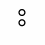
\includegraphics[]{img/reference/ref_03_offtype_symbol.png} \\ \hline
    \end{tabular}
\end{center}

%%% Local Variables: 
%%% mode: latex
%%% TeX-master: "rodin-doc"
%%% End: 
